\documentclass{article}

\usepackage[utf8]{inputenc}
\usepackage[MeX]{polski}
\usepackage{lmodern}
\usepackage[T1]{fontenc}
\usepackage{indentfirst}
\usepackage[letterpaper,top=2cm,bottom=2cm,left=3cm,right=3cm,marginparwidth=1.75cm]{geometry}

% Useful packages
\usepackage{amsmath}
\usepackage{amssymb}
\usepackage{graphicx}
\usepackage[colorlinks=true, urlcolor=blue, linkcolor=black]{hyperref}
\usepackage{subcaption}
\usepackage{fancyhdr}
\usepackage{multicol}
\usepackage{float}
\pagestyle{fancy}
\fancyhf{} 
\fancyhead[L]{[MIOwAD] - raport MLP}
\fancyfoot[C]{\thepage}

\begin{document}

\title{
\large WYDZIAŁ MATEMATYKI I NAUK INFORMACYJNYCH \\
\large POLITECHNIKA WARSZAWSKA\\
\hrulefill \\
\LARGE Algorytmy genetyczne\\
\hrulefill \\
\large SPRAWOZDANIE}
\author{Kornel Tłaczała}

\maketitle
\tableofcontents
\newpage
\section*{AE1: Implementacja algorytmu genetycznego}
\addcontentsline{toc}{section}{AE1: Implementacja algorytmu genetycznego}
\subsection*{Cel}
Zaimplementowanie algorytmu genetycznego, który będzie w stanie rozwiązać problem optymalizacji funkcji. W tym przypadku celem jest znalezienie minimum dwóch funkcji:
\begin{enumerate}
    \item $f(x, y, z) = x^2 + y^2 + 2z^2$.
    \item funkcja Rastrigina
\end{enumerate}
\subsection*{Implementacja}
Model został zaimplementowany w języku Python. Trening przeprowadzany jest po wygenerowaniu populacji początkowej, która losowana jest z rozkładu jednostajnego wokół zera. Następnie, w każdej iteracji, wykonywane są następujące kroki:
\begin{enumerate}
    \item Selekcja rodziców - wybór osobników do reprodukcji. W tym przypadku zastosowano bardzo prostą selekcję. Wybierany jest pewien procent najlepszych osobników z populacji.
    \item Krzyżowanie - tworzenie nowych osobników poprzez krzyżowanie rodziców. W tej implementacji każdy rodzic tworzy dwóch potomków z każdym innym rodzicem. Krzyżowanie polega na wymianie części genotypów rodziców. Wykorzystana została tu metoda \texttt{one\_point\_crossover}, gdzie punkt krzyżowania jest losowany losowo.
    \item Mutacja - wprowadzenie losowych zmian w genotypie potomków, aby zwiększyć różnorodność populacji. Prowadzi to do powstania szumu i pozwala na przeszukiwanie całej przestrzeni rozwiązań
    \item Finalna selekcja - wybór najlepszych osobników z populacji potomnej. Zastosowano tutaj elityzm - procent najlepszych rodziców zawsze zostaje w populacji. Reszta miejsc jest uzupełniana przez najlepszych osobników.
\end{enumerate}

\subsection*{Wyniki}
Dla obu funkcji model był w stanie efektywnie znaleźć minimum. Oczywiście w przypadku obu funkcji minimum jest w zerze. Wyniki to zdecydowanie odzwierciedlają:
\begin{figure}[H]
    \centering
    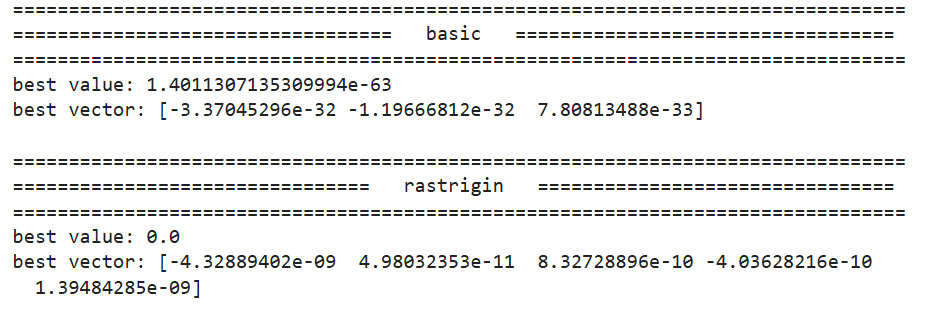
\includegraphics[width=0.8\textwidth]{img/ae1/results.png}
    \caption{Wyniki dla obu funkcji}
\end{figure}

\subsubsection*{Szybkość osiągania precyzji}
\begin{figure}[H]
    \centering
    \begin{subfigure}{0.45\textwidth}
        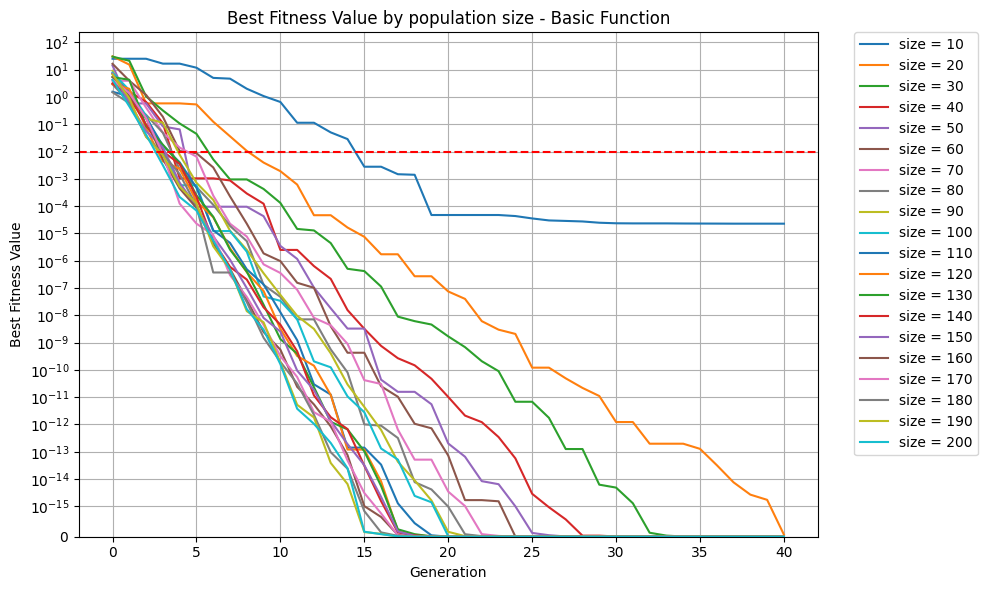
\includegraphics[width=\linewidth]{img/ae1/size_precision.png}
        \caption{Precyzja dla różnych rozmiarów populacji wg. epoki}
    \end{subfigure}
    \hfill
    \begin{subfigure}{0.45\textwidth}
        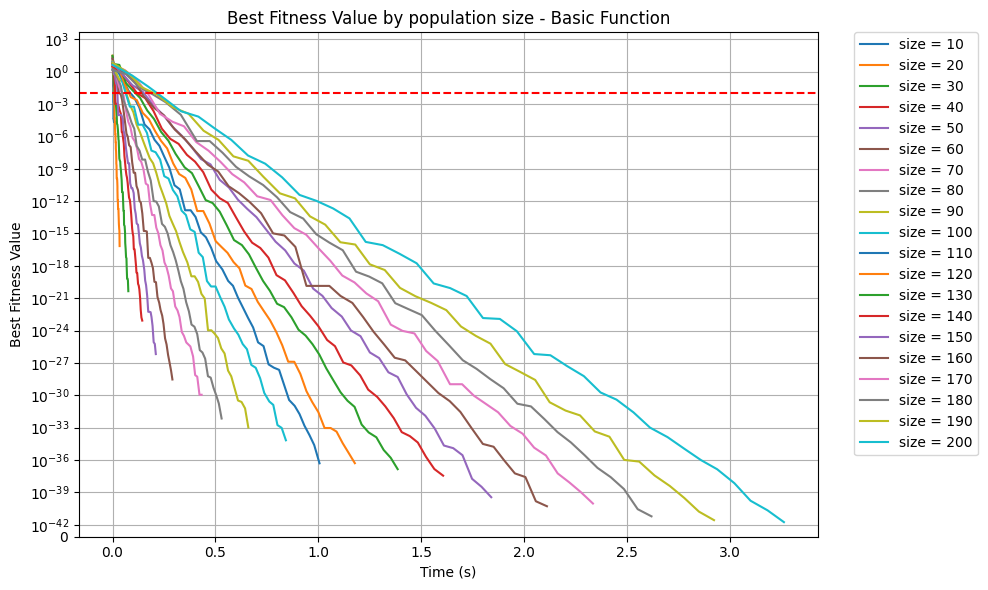
\includegraphics[width=\linewidth]{img/ae1/size_time.png}
        \caption{Czas osiągania precyzji dla różnych rozmiarów populacji}
    \end{subfigure}
    \caption{Zwykła funkcja kwadratowa - opłacalność rozmiaru populacji}
\end{figure}
Jak widać mniejsze populacje szybciej osiągają większą precyzję. Wynika to z tego, że złożoność algorytmu jest liniowa względem rozmiaru populacji. Jednakże, mniejsze populacje mogą nie być w stanie znaleźć minimum, ponieważ nie mają wystarczającej różnorodności genetycznej. Szczególnie widać to dla funkcji Rastrigina, gdzie mała populacja może łatwo utknąć w lokalnym minimum.

\subsubsection*{Zależność zbieżności od gęstości selekcji rodziców}
\begin{figure}[H]
    \centering
    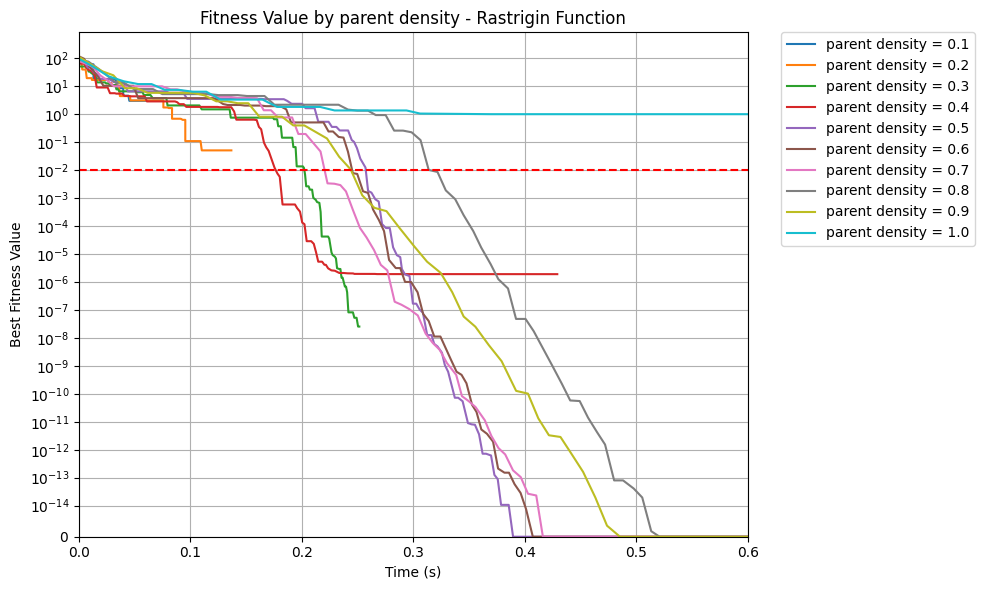
\includegraphics[width=0.8\textwidth]{img/ae1/parent_density.png}
    \caption{Zbieżność w zależności od gęstości selekcji rodziców}
\end{figure}
Jak widać, optymalne wartości gęstości selekcji rodziców są z przedziału $0.5 - 0.7$. Przy zbyt małej gęstości selekcji rodziców, populacja nie osiąga optymalnej precyzji. Zbyt duża gęstośc wydłuża natomiast działanie algorytmu.

\subsubsection*{Zależność zbieżności od skali mutacji}
\begin{figure}[H]
    \centering
    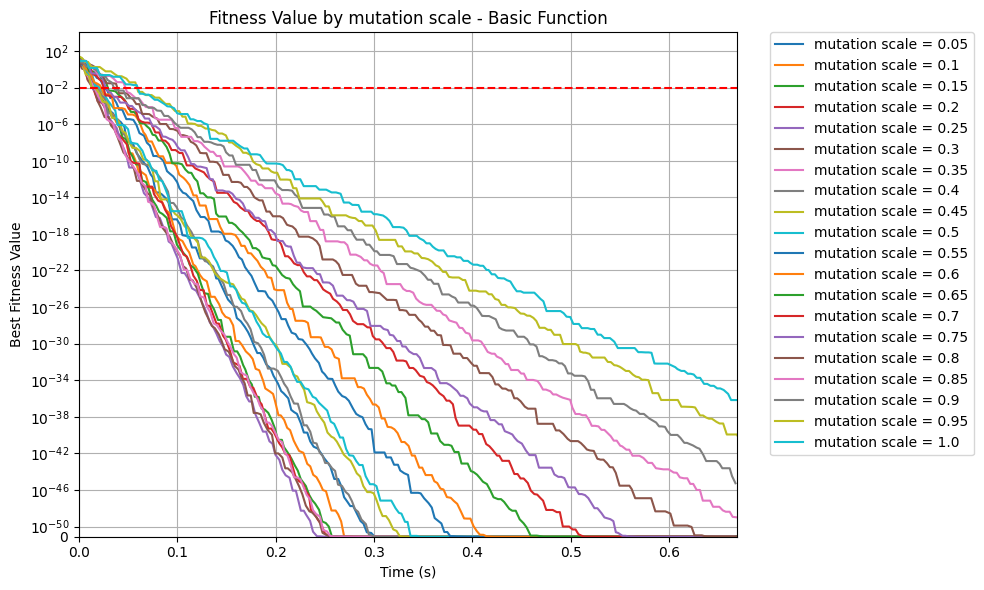
\includegraphics[width=0.8\textwidth]{img/ae1/mutation_scale.png}
    \caption{Zbieżność w zależności od skali mutacji}
\end{figure}
Najlepsze skale mutacji są z przedziału $0.05 - 0.4$.

\subsubsection*{Funkcja Rastrigina}
Funkcja Rastrigina jest funkcją o wielu minimach lokalnych, co sprawia, że jest trudna do optymalizacji. Na wykresie czerwone kropki oznaczają nową populację, niebieskie starą populację. Na zielono są dzieci starej populacji a na fioletowo ich mutacje. Dopiero teraz widać, dlaczego zbyt mały rozmiar populacji może zapobiec znalezieniu rozwiązania.
\begin{figure}[H]
    \centering
    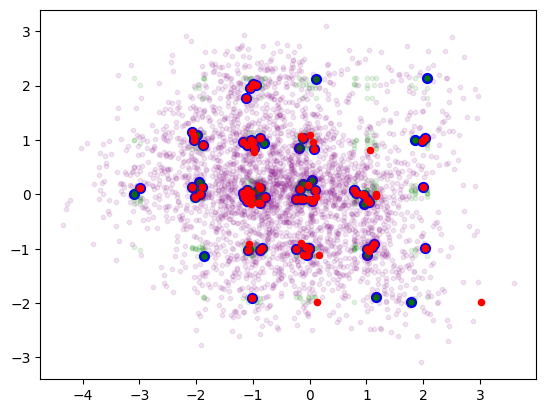
\includegraphics[width=0.7\textwidth]{img/ae1/rastrigin_distribution.png}
    \caption{Wizualizacja działania algorytmu na funkcji Rastrigina}
\end{figure}

\newpage

\section*{AE2: Wypełnianie koła prostokątami}
\addcontentsline{toc}{section}{AE2: Wypełnianie koła prostokątami}
\subsection*{Cel}
Celem zadania jest zaprojektowanie algorytmu, który maksymalizuje powierzchnię prostokątów umieszczonych wewnątrz koła o zadanym promieniu.  Algorytm powinien znaleźć taki układ prostokątów, aby suma ich pól była jak największa. Problem ten jest przykładem zadania optymalizacyjnego z ograniczeniami geometrycznymi i może być rozwiązywany m.in. z wykorzystaniem algorytmów ewolucyjnych.
\subsection*{Implementacja}
Od razu można zauważyć, że bardzo dużo miejsca w okręgu można stracić poprzez przestrzenie w które nie jest w stanie zmieścić się żaden nowy prostokąt. Warto układać prostokąty tak, aby do siebie przylegały. Najprostszym zatem rozwiązaniem okazało się umieszczenie prostokątów w kolumnach o jednolitym typie prostokąta. Genomem zatem można określić listę rodzajów prostokątów, które będą umieszczane w kolejnych kolumnach.
Przykładowe umieszczenie można zaobserwować na poniższym rysunku:
\begin{figure}[H]
    \centering
    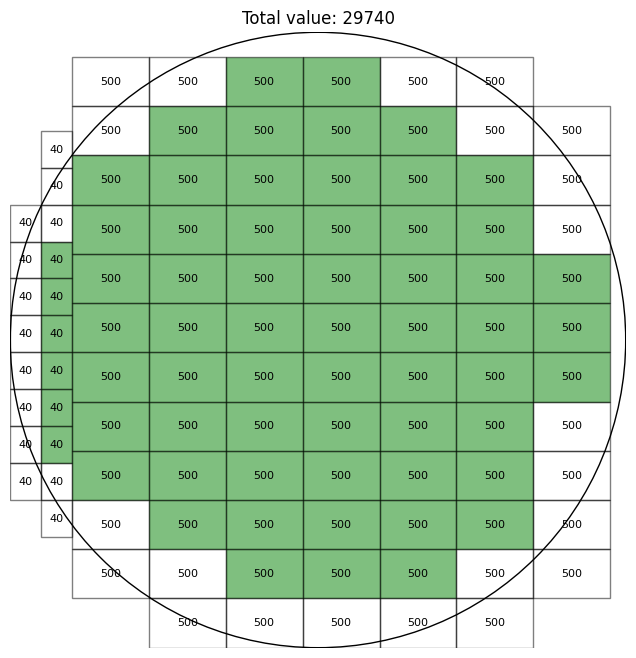
\includegraphics[width=0.8\textwidth]{img/ae2/rectangles_example.png}
    \caption{Przykładowe umieszczenie prostokątów w kole}
\end{figure}

\subsection*{Proces treningowy}
Trening przebiegał w sposób podobny do treningu algorytmu genetycznego z AE1. Wygenerowana została populacja początkowa, każdy osobnik (układ rodzajów prostokątów w kolumnach) jest oceniany poprzez obliczenie pola powierzchni prostokątów, które są w stanie zmieścić się w kole. Następnie, w każdej iteracji, wykonywane są następujące kroki:
\begin{enumerate}
    \item Selekcja rodziców - wybór osobników do reprodukcji. W tym przypadku zastosowano selekcję turniejową. Wybieramy pewien procent (przykładowo 10\%) osobników, którzy biorą udział w turnieju. Wybierany jest najlepszy osobnik z tego turnieju. Tak wybieramy rodzica nr. 1 oraz rodzica nr. 2.
    \item Krzyżowanie - tworzenie nowych osobników poprzez krzyżowanie rodziców. W tej implementacji każdy rodzic tworzy dwóch potomków z każdym innym rodzicem. Krzyżowanie polega na wymianie części genotypów rodziców. Wykorzystana została tu metoda \texttt{one\_point\_crossover}, gdzie punkt krzyżowania jest losowany losowo. Oczywiście, może się okazać, że kolumny potomka są zbyt szerokie lub zbyt wąskie. W takim przypadku nadmiar kolumn jest ucinany, a brakujące kolumny są uzupełniane losowymi rodzajami prostokątów.
    \item Mutacja - wprowadzenie losowych zmian w genotypie potomków, aby zwiększyć różnorodność populacji. Prowadzi to do powstania szumu i pozwala na przeszukiwanie całej przestrzeni rozwiązań. Mutacja polega na losowym przemieszaniu wszystkich kolumn potomka.
    \item Finalna selekcja - aby nie tracić jakości modelu najgorszy osobnik nowej populacji jest zastępowany przez najlepszego osobnika z poprzedniej populacji.
\end{enumerate}

\subsection*{Wyniki}

\subsubsection*{Koło o promieniu $r=800$}
Cel: osiągnięcie wartości $Value > 30000$.
\begin{figure}[H]
    \centering
    \begin{subfigure}{0.48\textwidth}
        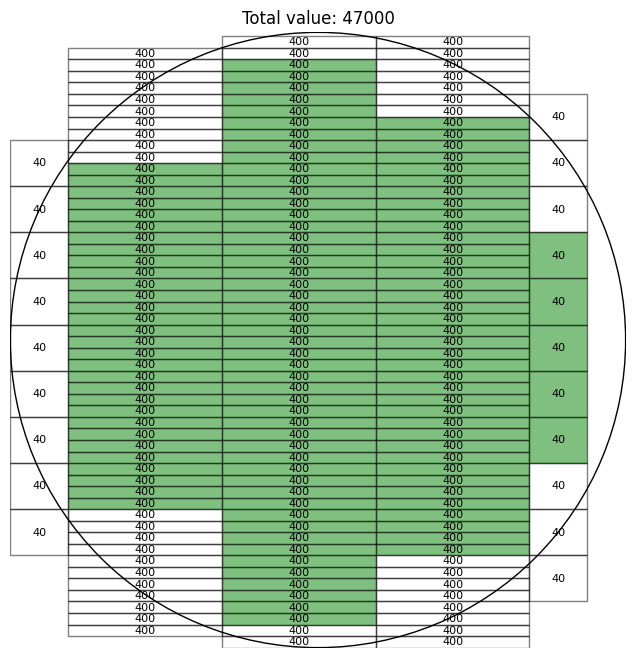
\includegraphics[width=\linewidth]{img/ae2/r800_fit.png}
        \caption{Najlepsze rozmieszczenie prostokątów}
    \end{subfigure}
    \hfill
    \begin{subfigure}{0.48\textwidth}
        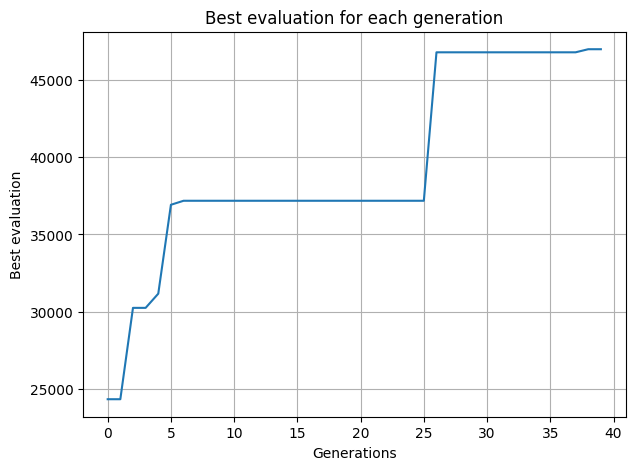
\includegraphics[width=\linewidth]{img/ae2/r800_history.png}
        \caption{Postęp treningu}
    \end{subfigure}
    \caption{Wyniki dla koła o promieniu $r=800$}
\end{figure}
\newpage

\subsubsection*{Koło o promieniu $r=850$}
Cel: osiągnięcie jak najwyższego wyniku.
\begin{figure}[H]
    \centering
    \begin{subfigure}{0.48\textwidth}
        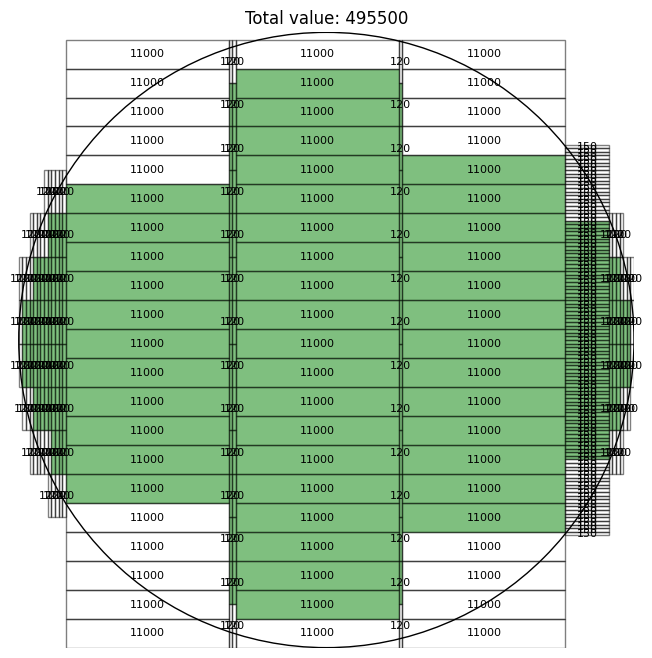
\includegraphics[width=\linewidth]{img/ae2/r850_fit.png}
        \caption{Najlepsze rozmieszczenie prostokątów}
    \end{subfigure}
    \hfill
    \begin{subfigure}{0.48\textwidth}
        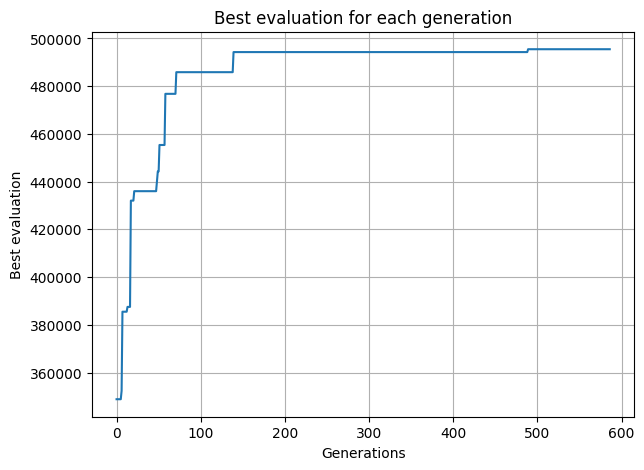
\includegraphics[width=\linewidth]{img/ae2/r850_history.png}
        \caption{Postęp treningu}
    \end{subfigure}
    \caption{Wyniki dla koła o promieniu $r=850$}
\end{figure}

\subsubsection*{Koło o promieniu $r=1000$}
Cel: osiągnięcie wartości $Value > 17500$.
\begin{figure}[H]
    \centering
    \begin{subfigure}{0.48\textwidth}
        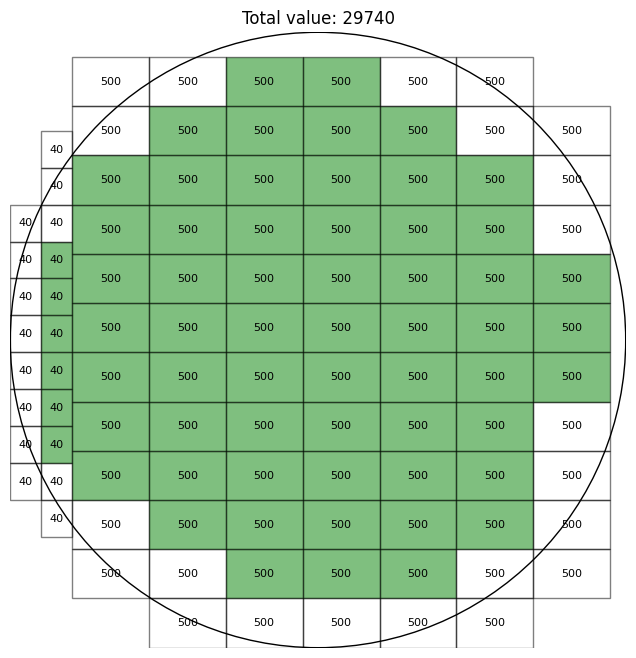
\includegraphics[width=\linewidth]{img/ae2/r1000_fit.png}
        \caption{Najlepsze rozmieszczenie prostokątów}
    \end{subfigure}
    \hfill
    \begin{subfigure}{0.48\textwidth}
        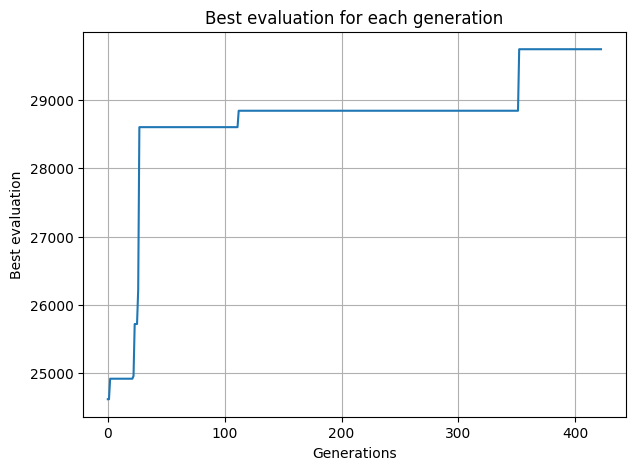
\includegraphics[width=\linewidth]{img/ae2/r1000_history.png}
        \caption{Postęp treningu}
    \end{subfigure}
    \caption{Wyniki dla koła o promieniu $r=1000$}
\end{figure}
\newpage

\subsubsection*{Koło o promieniu $r=1100$}
Cel: osiągnięcie wartości $Value > 25000$.
\begin{figure}[H]
    \centering
    \begin{subfigure}{0.48\textwidth}
        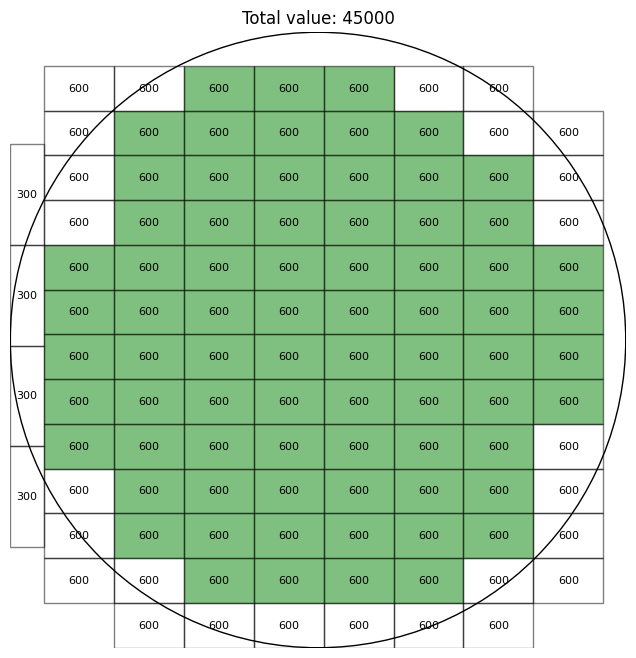
\includegraphics[width=\linewidth]{img/ae2/r1100_fit.png}
        \caption{Najlepsze rozmieszczenie prostokątów}
    \end{subfigure}
    \hfill
    \begin{subfigure}{0.48\textwidth}
        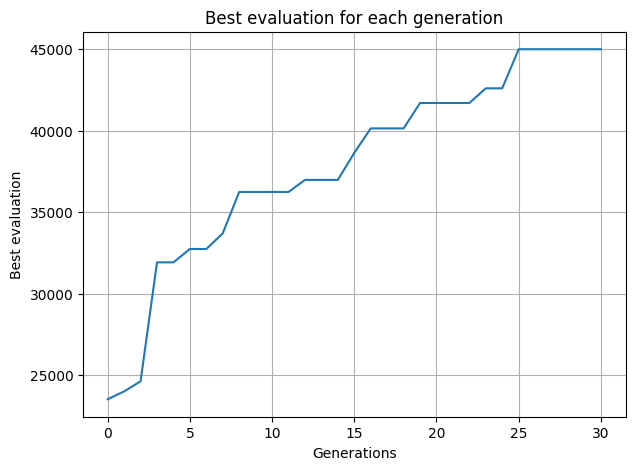
\includegraphics[width=\linewidth]{img/ae2/r1100_history.png}
        \caption{Postęp treningu}
    \end{subfigure}
    \caption{Wyniki dla koła o promieniu $r=1100$}
\end{figure}

\subsubsection*{Koło o promieniu $r=1200$}
Cel: osiągnięcie wartości $Value > 30000$.
\begin{figure}[H]
    \centering
    \begin{subfigure}{0.48\textwidth}
        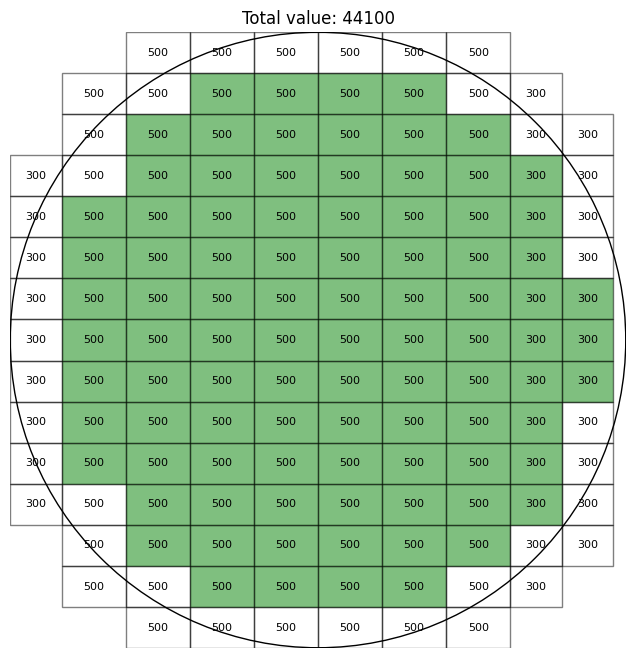
\includegraphics[width=\linewidth]{img/ae2/r1200_fit.png}
        \caption{Najlepsze rozmieszczenie prostokątów}
    \end{subfigure}
    \hfill
    \begin{subfigure}{0.48\textwidth}
        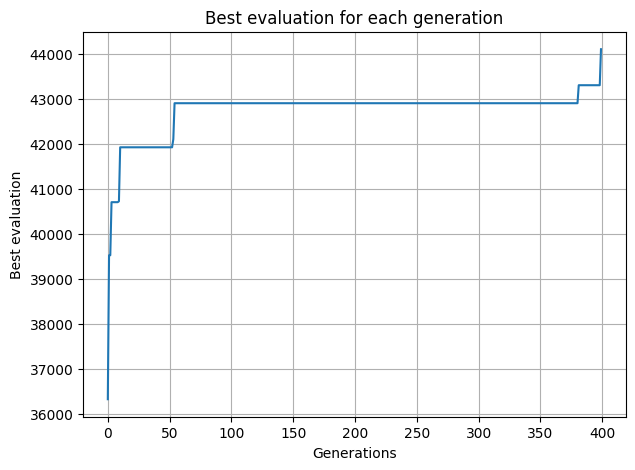
\includegraphics[width=\linewidth]{img/ae2/r1200_history.png}
        \caption{Postęp treningu}
    \end{subfigure}
    \caption{Wyniki dla koła o promieniu $r=1200$}
\end{figure}
\newpage

\section*{AE3: Optymalizacja wag sieci MLP z wykorzystaniem algorytmu genetycznego}
\addcontentsline{toc}{section}{AE3: Optymalizacja wag sieci MLP z wykorzystaniem algorytmu genetycznego}
\section*{Cel}
Celem zadania była optymalizacja wag sieci MLP (Multi-Layer Perceptron) z wykorzystaniem algorytmu genetycznego. W tym przypadku celem jest znalezienie wag, które pozwolą na jak najlepsze dopasowanie modelu do danych treningowych. Modele trenowane oraz oceniane były na zbiorach:
\begin{enumerate}
    \item square-simple (problem regresji jednowymiarowej)
    \item multimodal-large (problem regresji jednowymiarowej)
    \item iris (problem klasyfikacji)
    \item auto\_mpg (problem regresji wielowymiarowej)
\end{enumerate}

\section*{Implementacja}
Do implementacji modelu zosała wykorzystana już istniejąca struktura sieci MLP. Osobnikiem w populacji jest zmodyfikowany obiekt modelu MLP, tak zwany EvoMLP. Wagi oraz biasy sieci są traktowane jako genotyp osobnika. Osobnik jest oceniany przy użyciu natywnej funkcji straty modelu, określanej przy jego inicjalizacji. W przypadku regresji, funkcją oceny jest błąd średniokwadratowy (MSE), a w przypadku klasyfikacji - entropia krzyżowa (cross-entropy). Zadaniem jest zminimalizowanie wartości funkcji straty na zbiorze treningowym dla najlepszego osobnika w populacji.
\section*{Proces treningowy}
Wygenerowanie populacji początkowej było bardzo naturalnym krokiem, ponieważ domyślnie model MLP jest inicjalizowany z losowymi wagami i biasami. Następnie, w każdej iteracji, wykonywane są następujące kroki:
\begin{enumerate}
    \item Selekcja rodziców - wybór osobników do reprodukcji. Zastosowano tu selekcję tureniejową, tak jak w AE2. Wybierany jest pewien procent najlepszych osobników z populacji, którzy biorą udział w turnieju. Wybierany jest najlepszy osobnik z tego turnieju. Tak wybieramy rodzica nr. 1 oraz rodzica nr. 2. którzy tworzą parę.
    \item Krzyżowanie - tworzenie nowych osobników poprzez krzyżowanie rodziców. W tej implementacji każdy rodzic tworzy dwóch potomków z każdym innym rodzicem. Krzyżowanie polega na pobraniu jednej wagi oraz biasu dla losowego neuronu od drugiego rodzica. Daje to możliwość szybkiej, gwałtownej zmiany predykcji przez osobnika. Zazwyczaj taka zmiana jest niekorzystna, natomiast czasem może ona prowadzić do znacznej poprawy oceny modelu, co jest wypadkową znalezienia lepszego dopasowania do skomplikowanych danych. Szczególnie dobrze widać to na zbiorze multimodal-large.
    \item Mutacja - tutaj pomysłów było dużo. Pierwsze dwa polegały na zmianie wielu wag naraz przy jednym neuronie, lub zmianie wag na całej warstwie na raz. Okazały się one jednak nieskuteczne, ponieważ prawie nigdy nie powodowały korzystnej mutacji, ewaluacja modelu często stawała w miejscu. Ostatecznie zaimplementowana została mutacja, która dla wybranego neuronu mnoży jego wagę oraz bias przez losową wartość bliską 1. Parametr tej bliskości - \texttt{mutation\_strength} można dosyć swobodnie dobierać podczas procesu treningowego
    \item Finalna selekcja - trafiały tutaj 4 grupy osobników. Wszyscy osobnicy z poprzedniej generacji, wszystkie dzieci, dodatkowo zmutowani rodzice oraz dodatkowo zmutowane dzieci. Bardzo ważne okazało się pozostawianie 10\% najlepszych wygenerowanych osobników. Gwarantowało to stabilność modelu i pozwalało na uniknięcie regresji jakościowej. Model okazał się dosyć odporny na spadek różnorodności genetycznej. Duża liczba mutacji w każdej generacji pozwalała na wygenerowanie odmiennych osobników, potencjalnie troszkę lepszych niż rodzice. Ostatecznie, oprócz 10\% najlepszych osobników reszta kandydatów była wybierana z rozkładu prawdopodobieństwa proporcjonalnego do ich oceny. Oznacza to, że im lepszy osobnik, tym większa szansa, że zostanie wybrany do kolejnej generacji.
\end{enumerate}
\subsection*{Wyniki}
\subsubsection*{Square-simple}

\begin{figure}[H]
    \centering
    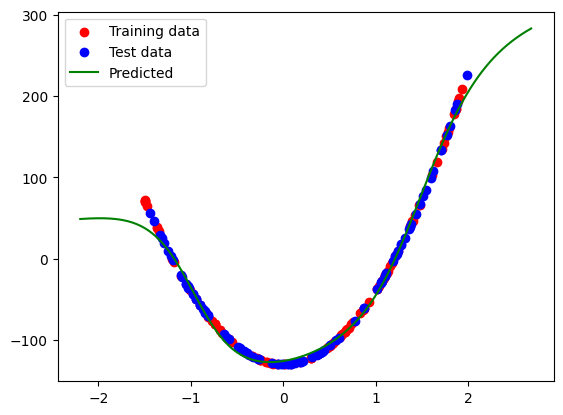
\includegraphics[width=\textwidth]{img/ae3/square-simple_fit.png}
    \caption{Dopasowanie modelu EvoMLP do zbioru square-simple}
\end{figure}
Dla tego prostego zbioru udało się osiągnąć zbliżone dopasowanie po około 600 epokach. Po 900 epokach wartość funkcji straty wyniosła $MSE = 37.16$. Jest to oczywiście wynik nieporównywalnie gorszy niż ten osiągany przez wsteczną propagację błędu, jednak satysfakcjonujące jest odwzorowanie przez algorytm kształtu funkcji w jej dziedzinie
\newpage

\subsubsection*{Iris}
Zadanie to jest problemem klasyfikacji 3-klasowej. Dla porównania, wytrenowany został również model MLP przy użyciu wstecznej propagacji błędu. Osiągnął on F1-score na poziomie 0.97, co jest bardzo dobrym wynikiem. Wyraźnie widoczne było jednak, że mimo zastosowania różnych architektur sieci model nie był wstanie zejść poniżej $cross\_entropy = 0.06$

\begin{figure}[H]
    \centering
    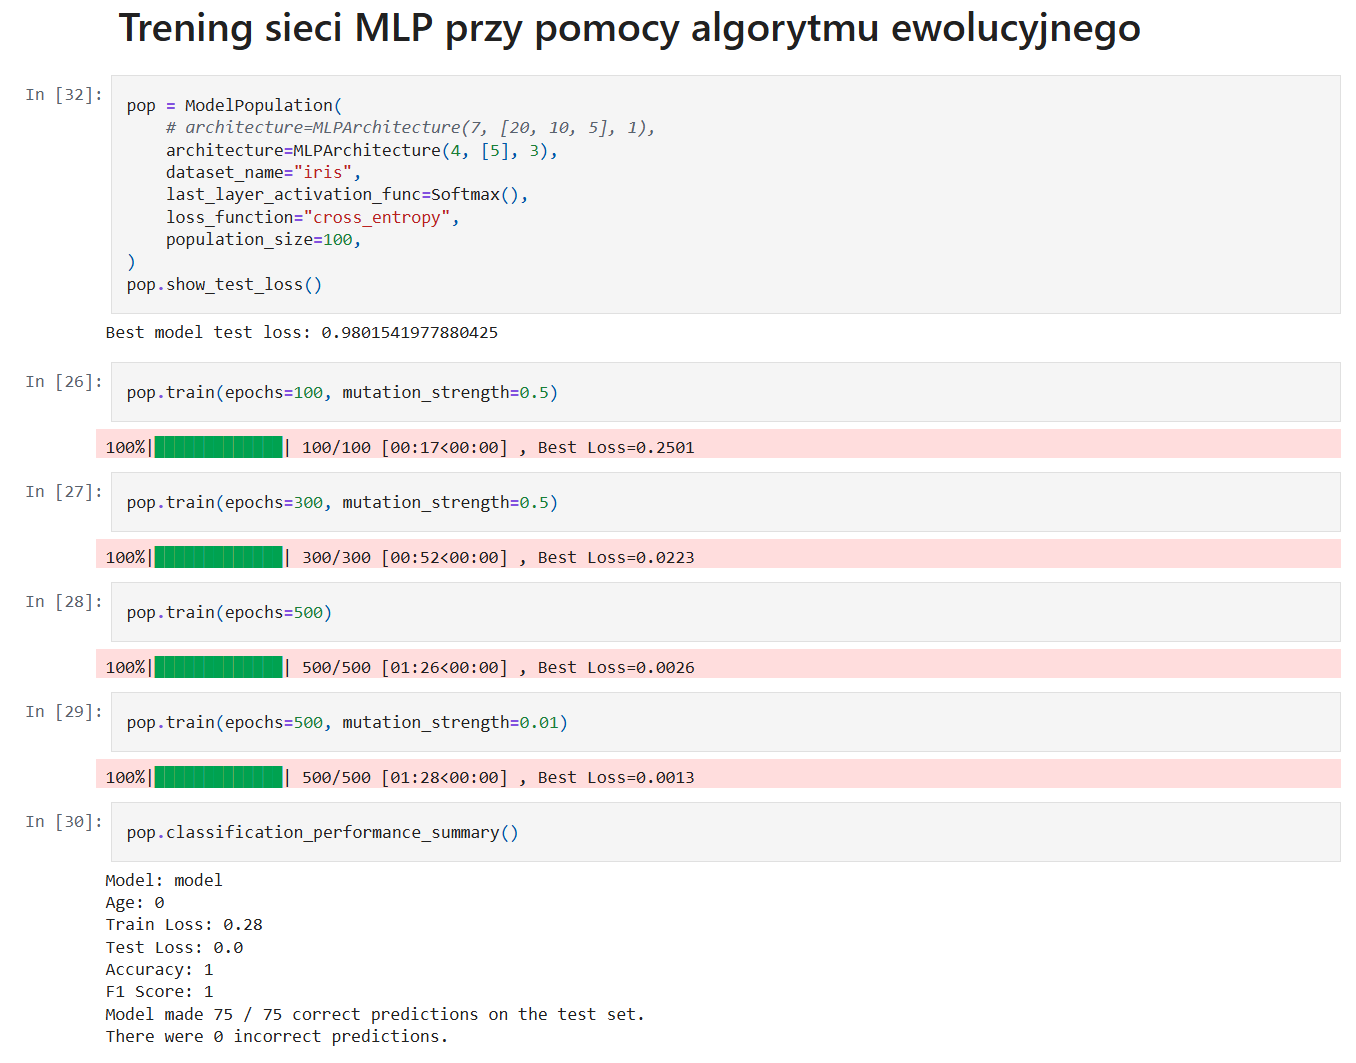
\includegraphics[width=\textwidth]{img/ae3/iris_training.png}
    \caption{Proces treningowy modelu EvoMLP na zbiorze iris}
\end{figure}

Dla algorytmu ewolucyjnego szczególne korzyści przyniósł trening z większą siłą mutacji. Pozwolił on osiągnąć wyraźnie niższą wartość funkcji straty (~0.001). Algorytm osiągnął wynik \texttt{F1-score = 1}, co jest lepszym wynikiem niż ten osiągnięty przez MLP z backpropagacją.

\subsubsection*{Auto MPG}

Zaskakująco dobrze model EvoMLP poradził sobie z tym zbiorem danych. Jest to zbiór regresji wielowymiarowej, gdzie celem jest przewidywanie zużycia paliwa w samochodach na podstawie ich parametrów technicznych. Zbiór ten zawiera 7 cech wejściowych i jedną cechę wyjściową (zużycie paliwa).

Zbiór ten wymagał usunięcia kilku wierszy z brakującymi danymi. Dopiero to pozwoliło na wytrenowanie modelu, zarówno MLP jak i Populacji EvoMLP. 

Co ciekawe, algorytm ewolucyjny osiągnął lepszy wynik niż klasyczna wsteczna propagacja błędu, nawet przy zastosowaniu zaawansowanych technik takich jak RMSprop, uczenie z momentem, regularyzacja, adaptacyjna zmiana współczynnika nauczania czy zatrzymywanie procesu nauczania w przypadku przeuczania. Mimo tych usprawnień, model trenowany backpropagacją nie był w stanie zejść poniżej $MSE = 6.0$. Algorytm ewolucyjny natomiast ostatecznie osiągnął $MSE < 4.5$, co stanowi zauważalną poprawę jakości predykcji na tym zbiorze danych.

\begin{figure}[H]
    \centering
    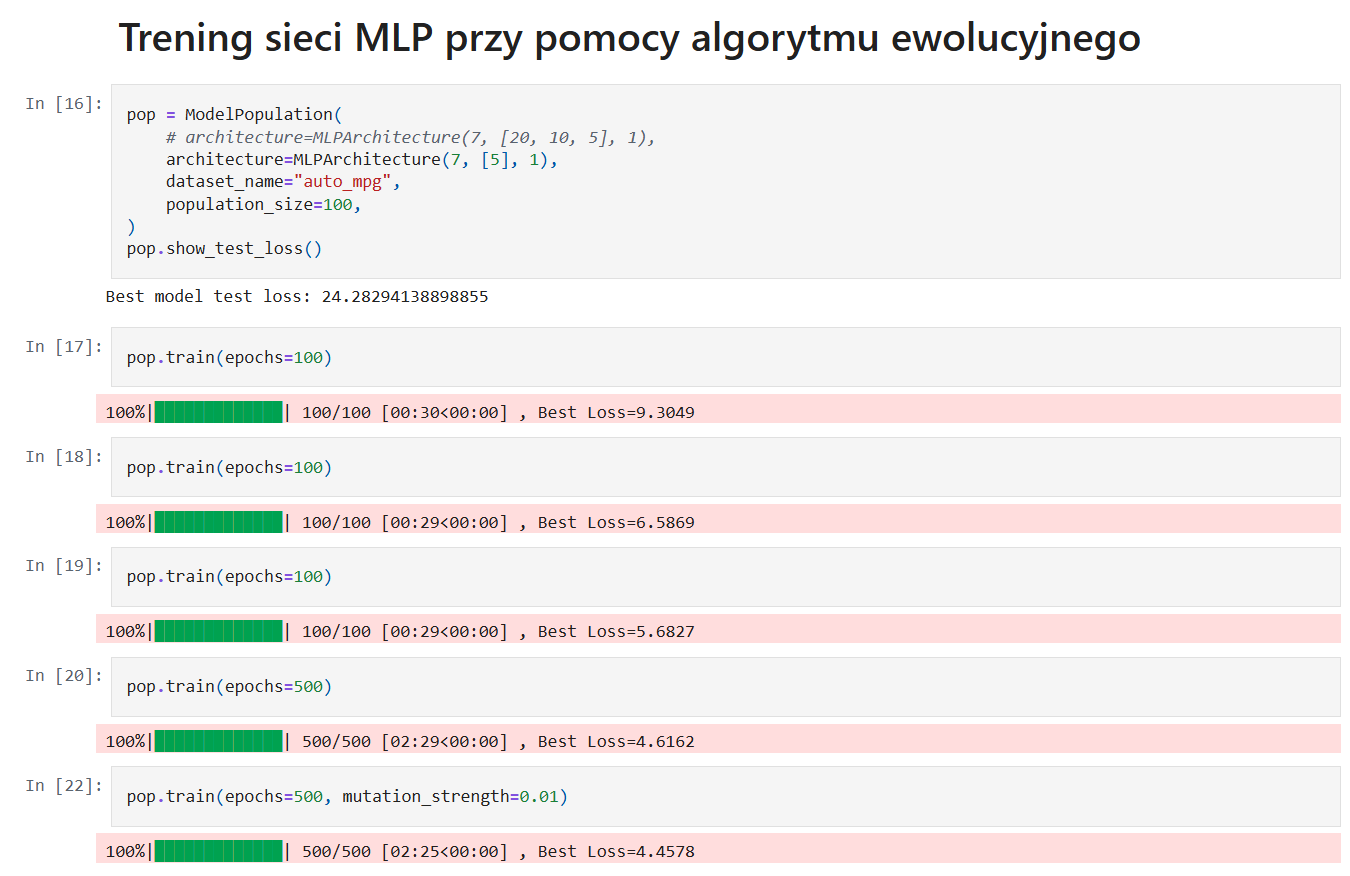
\includegraphics[width=\textwidth]{img/ae3/auto_mpg_training.png}
    \caption{Proces treningowy modelu EvoMLP na zbiorze auto mpg}
\end{figure}
\newpage

\subsubsection*{Multimodal-large}
Największym zaskoczeniem podczas testowania algorytmu ewolucyjnego była jego zdolność do radzenia sobie z bardzo skomplikowanym zbiorem multimodal-large. Jest to zbiór regresji jednowymiarowej, gdzie celem jest przewidywanie wartości funkcji o wielu minimach lokalnych.
\begin{figure}[H]
    \centering
    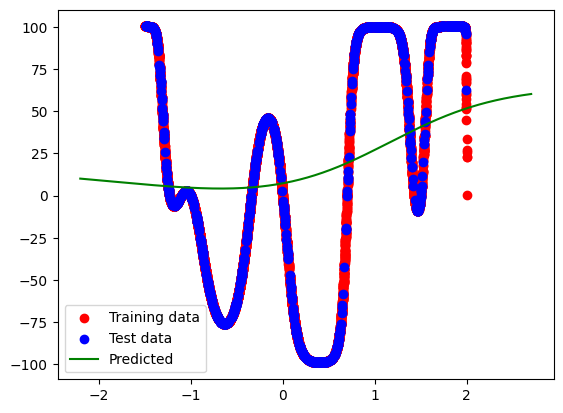
\includegraphics[width=\textwidth]{img/ae3/mml1.png}
    \caption{Początkowe dopasowanie populacji EvoMLP do zbioru multimodal-large}
\end{figure}
Jak widać, zadaniem jest tutaj predykcja wartości skomplikowanej funkcji, wymagającej agresywnych zmian wag podczas procesu treningowego. Dużo w procesie treningowym pomagało regularne dostosowywanie siły mutacji. Okresowe zwiększanie siły mutacji pozwalało na znalezienie lepszego rozwiązania, wyraźnie odmiennego od obecnych w populacji, co pozwoliło dopasować się do nieregularnego kształtu funkcji.
Następnie zmniejszenie siły mutacji pozwalało na bliższe dopasowanie znalezionego rozwiązania i przyśpieszało postęp.

\newpage
\subsubsection*{Historia procesu treningowego modelu EvoMLP do zbioru multimodal-large}
\begin{figure}[H]
    \centering
    \begin{subfigure}{0.32\textwidth}
        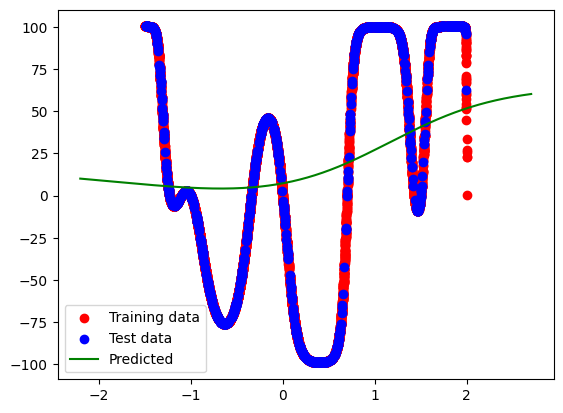
\includegraphics[width=\linewidth]{img/ae3/mml1.png}
        \caption{Epoka 0}
    \end{subfigure}
    \hfill
    \begin{subfigure}{0.32\textwidth}
        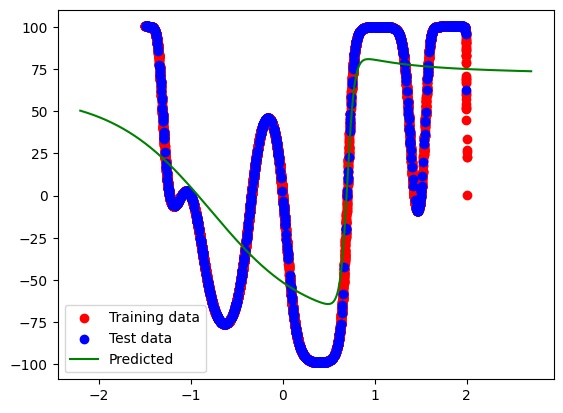
\includegraphics[width=\linewidth]{img/ae3/mml2.png}
        \caption{Epoka 200}
    \end{subfigure}
    \hfill
    \begin{subfigure}{0.32\textwidth}
        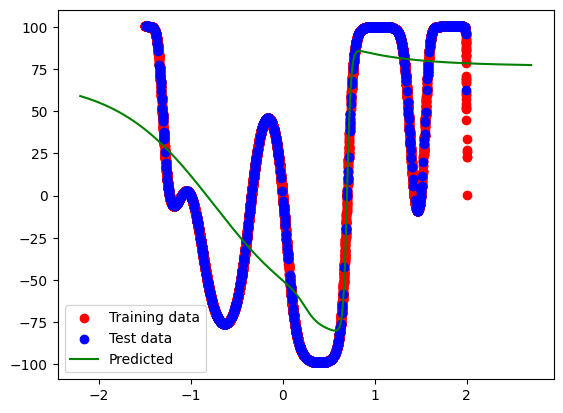
\includegraphics[width=\linewidth]{img/ae3/mml3.png}
        \caption{Epoka 300}
    \end{subfigure}
\end{figure}

\begin{figure}[H]
    \centering
    \begin{subfigure}{0.32\textwidth}
        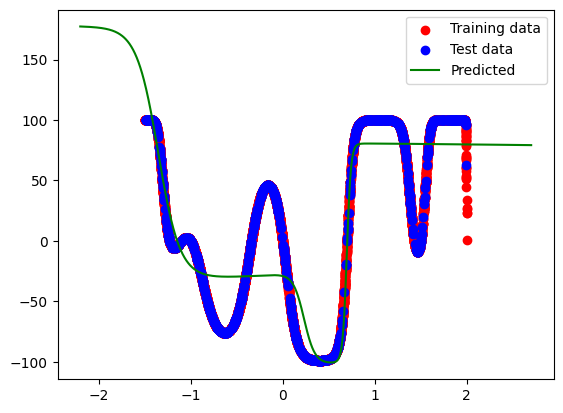
\includegraphics[width=\linewidth]{img/ae3/mml4.png}
        \caption{Epoka 800}
    \end{subfigure}
    \hfill
    \begin{subfigure}{0.32\textwidth}
        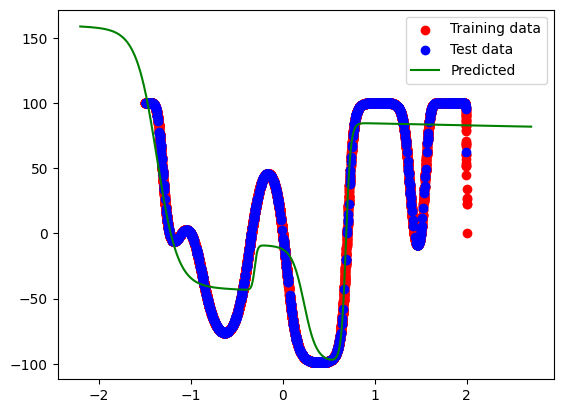
\includegraphics[width=\linewidth]{img/ae3/mml5.png}
        \caption{Epoka 1200}
    \end{subfigure}
    \hfill
    \begin{subfigure}{0.32\textwidth}
        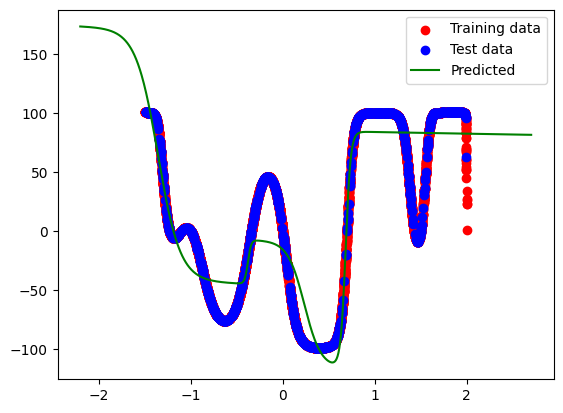
\includegraphics[width=\linewidth]{img/ae3/mml6.png}
        \caption{Epoka 1300}
    \end{subfigure}
\end{figure}

\begin{figure}[H]
    \centering
    \begin{subfigure}{0.32\textwidth}
        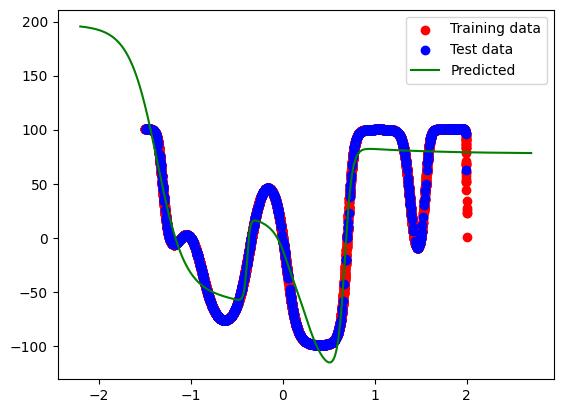
\includegraphics[width=\linewidth]{img/ae3/mml7.png}
        \caption{Epoka 1900}
    \end{subfigure}
    \hfill
    \begin{subfigure}{0.32\textwidth}
        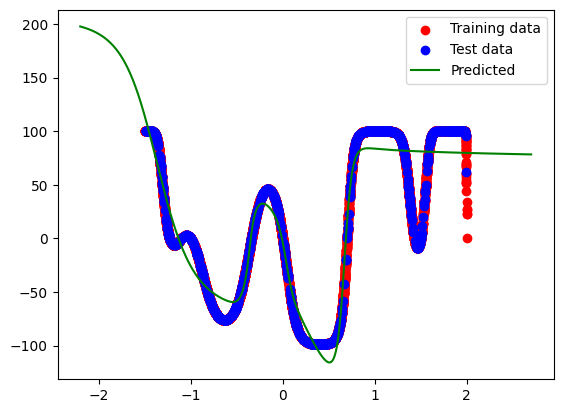
\includegraphics[width=\linewidth]{img/ae3/mml8.png}
        \caption{Epoka 2900}
    \end{subfigure}
    \hfill
    \begin{subfigure}{0.32\textwidth}
        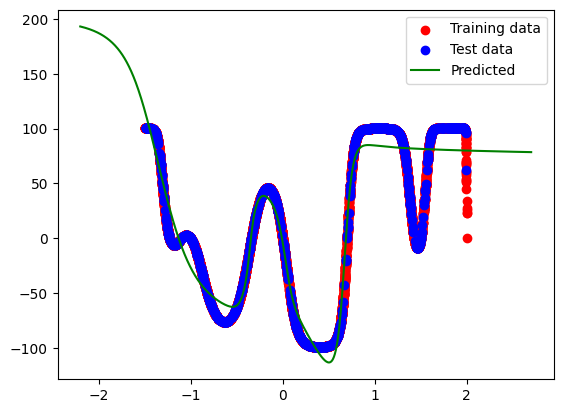
\includegraphics[width=\linewidth]{img/ae3/mml9.png}
        \caption{Epoka 3300}
    \end{subfigure}
\end{figure}

Zdecydowaną wadą tego algorytmu jest jego czas działania. Lepszą ostateczną skuteczność zapewniają większe populacje, które z kolei wolniej przeszukują przestrzeń rozwiązań, gdyż generują dużo podobnych osobników. 

\newpage
\subsubsection*{Ostateczne dopasowanie na zbiorze multimodal-large}
\begin{figure}[H]
    \centering
    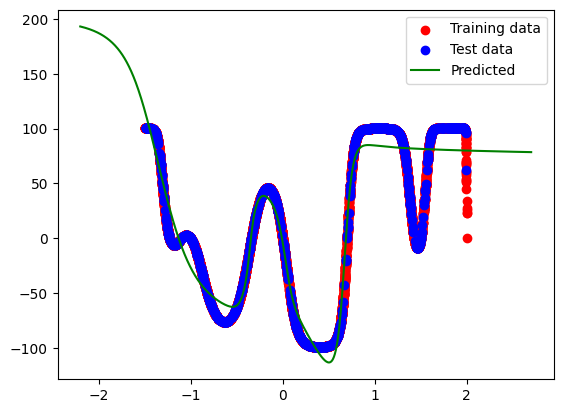
\includegraphics[width=\textwidth]{img/ae3/mml9.png}
    \caption{Ostateczne dopasowanie modelu EvoMLP do zbioru multimodal-large}
\end{figure}

\end{document}
